\subsection{Bestimmung der Offsetspannung}
Aus den gemessenen Spannungen $U_i$ bei ausgeschaltetem Magnetstrom lässt sich die Offsetspannung über
\begin{align*}
  \delta U=\frac{1}{5}\sum_i (U_{i,+}-U_{i,-})
\end{align*}
berechnen. Mit dem Fehler von $0,1$ auf jede einzelne Messung folgt mit gaußscher Fehlerfortpflanzung
\begin{align*}
  \delta U=4.40\pm 0.03.
\end{align*}
Von allen gemessenen Spannungen wird dieser Wert abgezogen.

\subsection{Kalibration des Spektrometers}
An das aufgenommene Emissionspektrum von Barium in der Feinmessung wird eine Überlagerung aus zwei Gaußkurven mit zusätzlichem Offset
\begin{align*}
  N(U)=A_0+A_1\exp \left(-\frac{(U-\mu_1)^2}{\sigma_1^2}\right) +A_2\exp\left(-\frac{(U-\mu_2)^2}{\sigma_2^2} \right)
\end{align*}
angepasst. Das Ergebnis ist
\begin{align*}
  A_0&=11\pm 2\\
  A_1&=157\pm 11\\
  A_2&=55\pm 6\\
  \mu_1&=153,52 \pm 0,05\\
  \mu_1&=157,6 \pm 0,1\\
  \sigma_1&=0,9 \pm 0,1\\
  \sigma_1&=0,7 \pm 0,2.
\end{align*}
Die graphische Auftragung ist in Abbildung \ref{fig:ba_fein} zu sehen.
\begin{figure}[h]
  \centering
  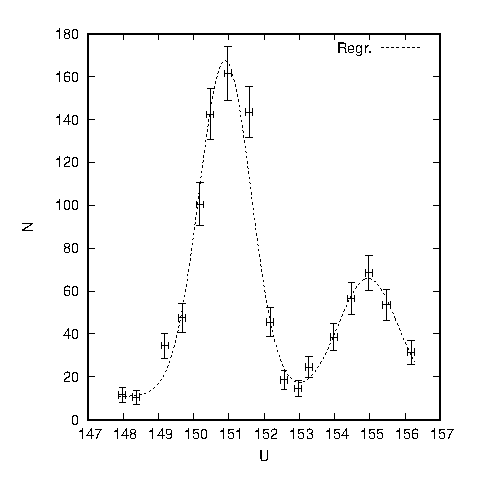
\includegraphics[width=0.7\textwidth]{data/Ba_fein.eps}
  \caption{Aufgezeichnetes Emissionsspektrum von Barium in Feinmessung}
  \label{fig:ba_fein}
\end{figure}

Die erste Emissionslinie entspricht der K-Linie, die zweite entspricht einer Überlagerung von drei L-Linien. Die (mittlere) Bindungsenergie von Elektronen aus der K- und L-Schale sind
\begin{align*}
  \epsilon_K&=0,07327020982\\
  \epsilon_L&=0,01099904421.
\end{align*} 
Der beobachtete $\beta^-$-Übergang hat eine Energie von
\begin{align*}
  \delta\epsilon=1,29483633.
\end{align*}
Der Impuls der Elektronen kann somit über 
\begin{align*}
  \eta=\sqrt{(\delta\epsilon-\epsilon+1)^2-1}
\end{align*}
 berechnet werden. Es folgt
\begin{align*}
  \eta_K&=1,983773179\\
  \eta_L&=2,053268796.
\end{align*}
Unter Hinzunahme des Datenpunktes $U=0 \pm 0,1$, $\eta=0$ wird die Kalibrationsgerade 
\begin{align*}
  \eta(U)=aU+b
\end{align*}
angepasst. Die Parameter sind
\begin{align*}
  a&=0,0130 \pm 0,0001\\
  b&=0,00 \pm 0,01.
\end{align*}
Die Funktion sowie die Daten sind in Abbildung \ref{fig:kal} zu sehen.
\begin{figure}[h]
  \centering
  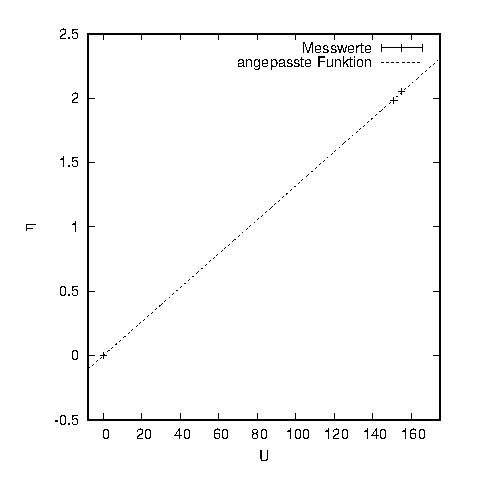
\includegraphics[width=0.7\textwidth]{data/kal.eps}
  \caption{Kalibrationskurve für Zusammenhang von Hallspannung und Elektronenimpuls}
  \label{fig:kal}
\end{figure}
